To validate our approach we train a model on the proposed dataset using both image and text data and compare it to text-only models. We choose the task of reconstructing the substituted utterance as visual signal is clearly beneficial in such setting.

\subsection{Model architecture}

We choose a pre-trained BLIP \cite{blip} model for experiments as it is one of the best open source models utilising both visual and text modalities and has a handy interface in LAVIS library \cite{lavis}. The model consists of a visual transformer \cite{vit} for image encoding and a BERT \cite{bert} with a language modeling head for text decoding, both initialised from a BLIP checkpoint. Training details shown in Appendix C.

\medskip

To validate the composed dataset we finetuned two BLIP models from a pre-trained checkpoint. These models consist of ViT-B/16 image encoder and BERT text decoer with 12 layers, 12 attention heads, hidden size of 768, intermediate size of 3072, and GeLU activations \cite{gelu}. Total number of parameters is 224M.


\subsection{Evaluation}

For evaluation we use 128 well annotated samples by both us and the assessors. For each trained model we choose the best checkpoint using validation metrics and use it to compute metrics on the test split. We compare BLIP finetuned on the proposed dataset to zero-shot performance of a distilled BlenderBot 400M \cite{blenderbot} and BLIP finetuned in text-only setting. We choose BLEU \cite{bleu} with n-grams lengths from 1 to 4 as quality metrics and also report perplexity for the models we trained. During evaluation we use beam search sampling with 3 beams. We also divide the test split of the dataset into parts corresponding to the source dialog corpuses and report the metrics for each of them in Table \ref{table:test_metrics_by_source} and for the whole set in Table \ref{table:test_metrics}.

\subsection{Generation examples}

Figure \ref{fig:examples} show some examples of model generation results. We find that the model finetuned using visual data uses that information in its answers as opposed to the one finetuned using constant visual inputs. As we have only one ground truth label for one sample sometimes model outputs do not exactly align with them, but usually make sense and come close.

\begin{figure}
    \centering
    % TODO: uncomment
    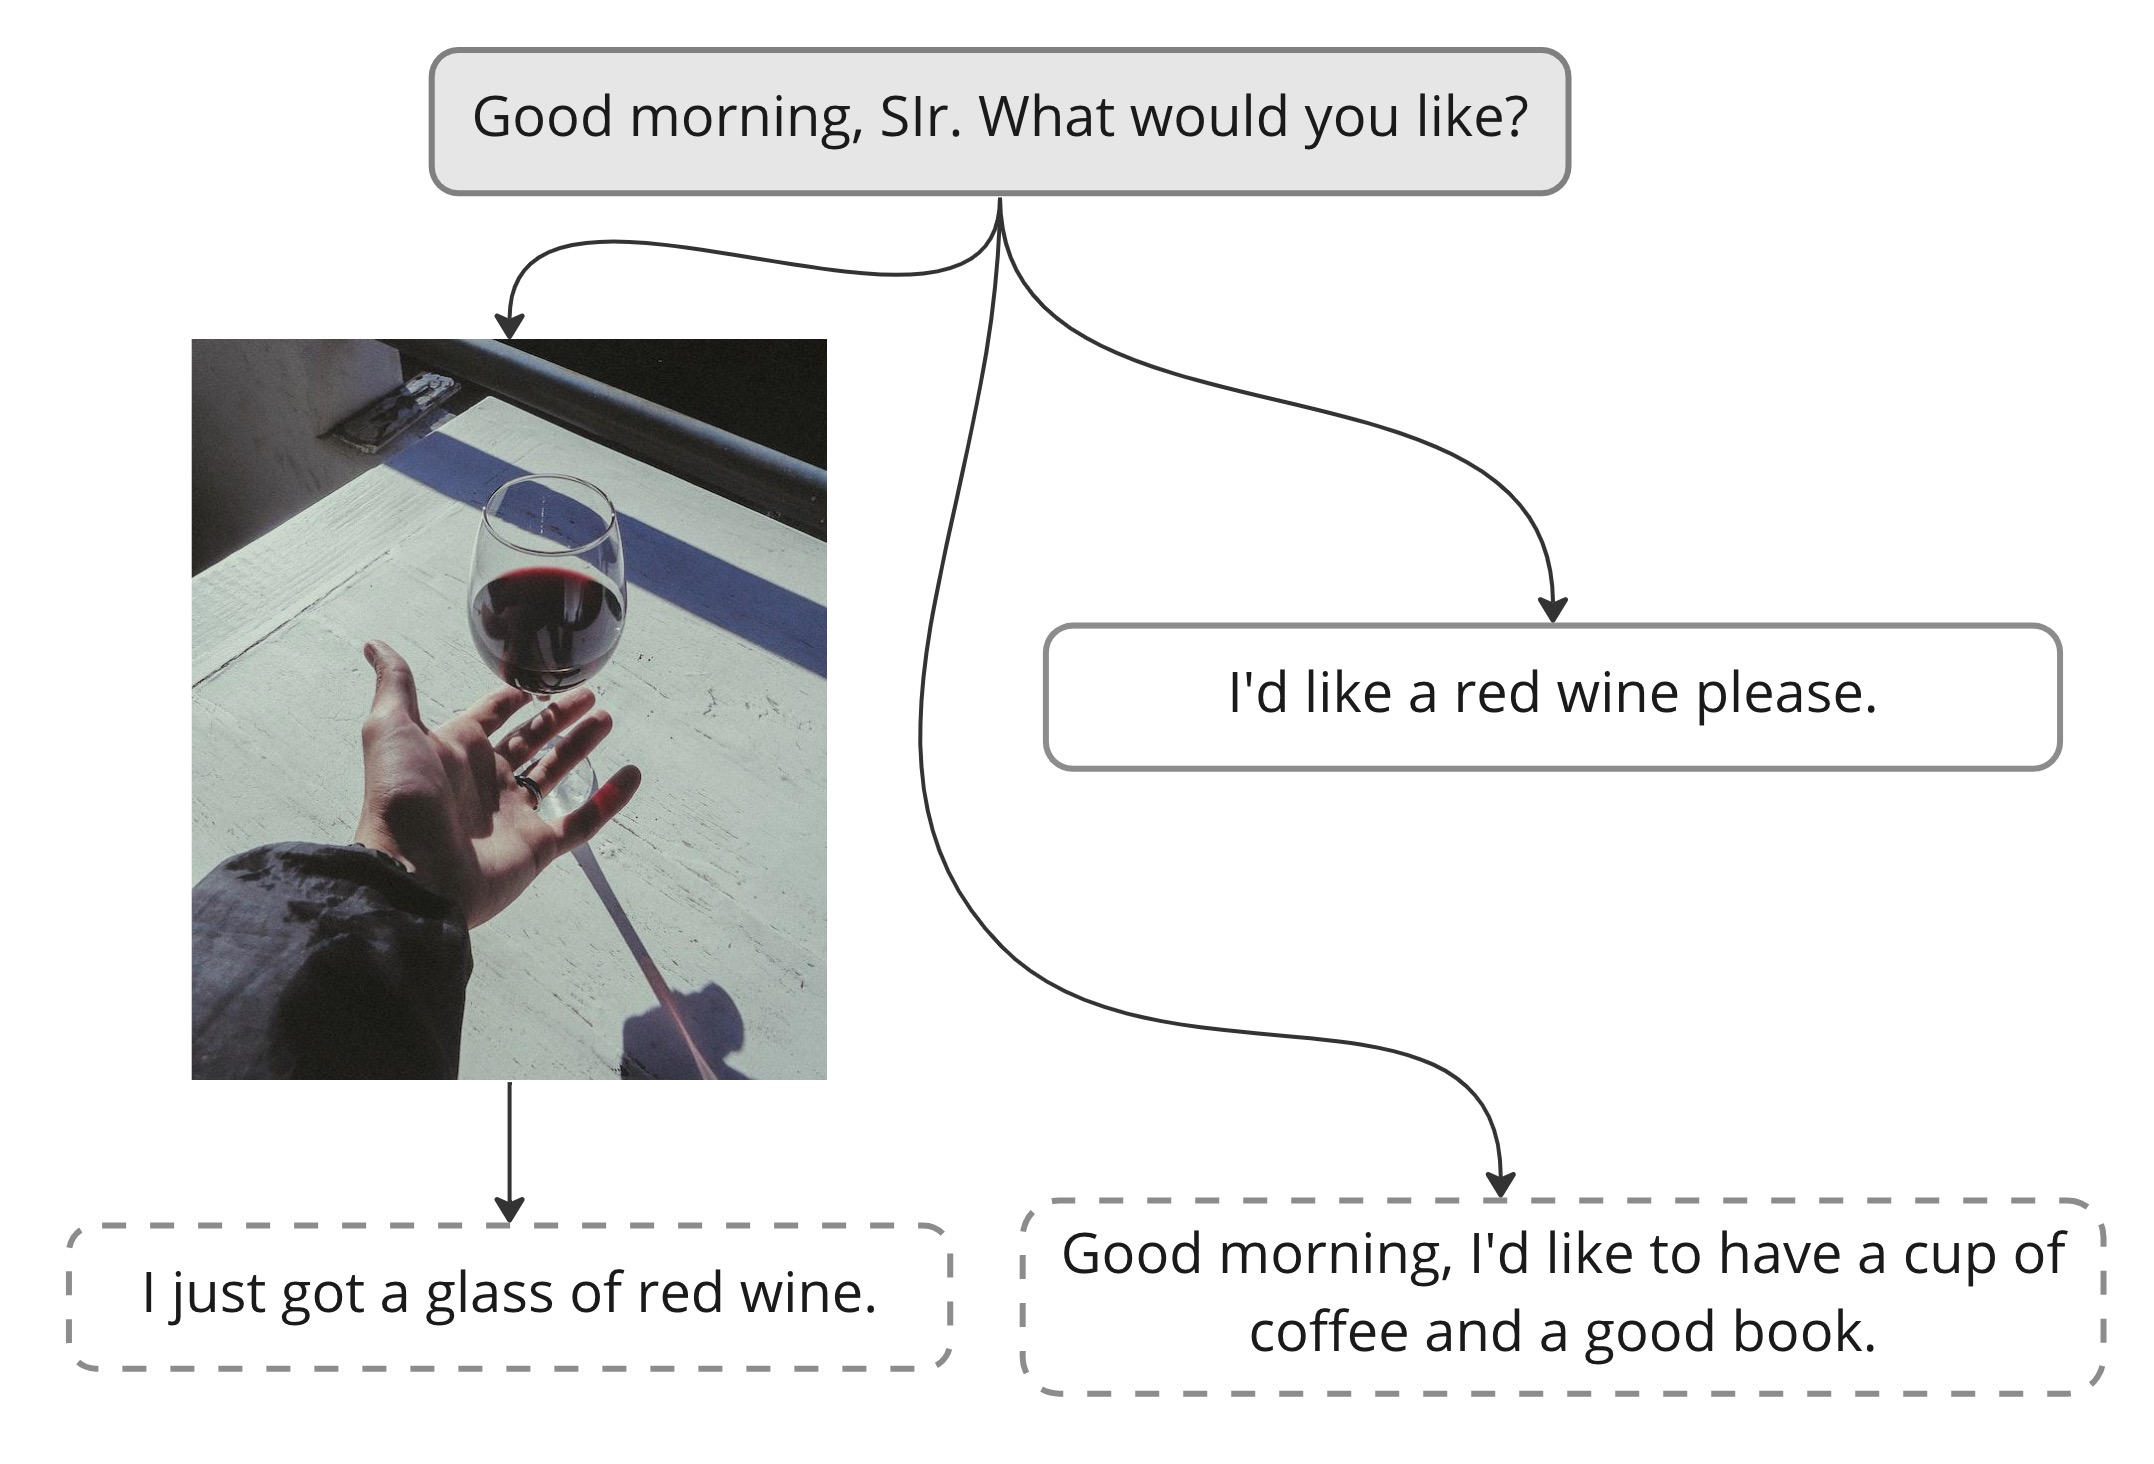
\includegraphics[width=0.49\linewidth, viewport=0 0 2154 1464]{example1.jpg}
    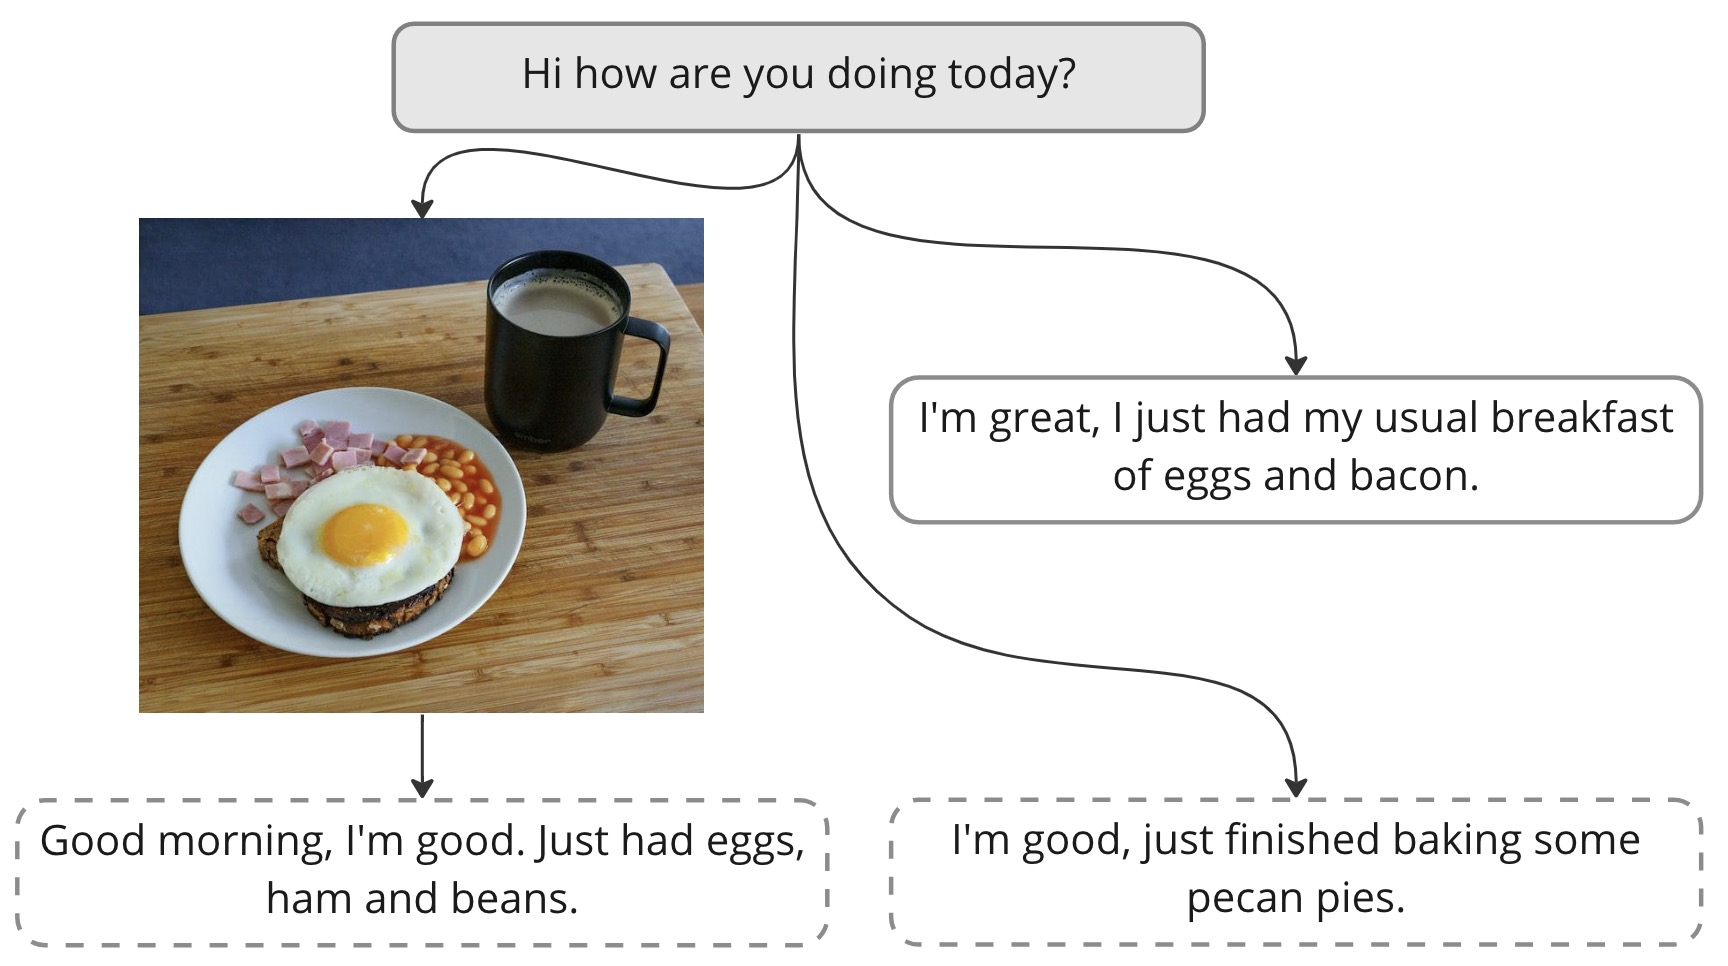
\includegraphics[width=0.49\linewidth, viewport=0 0 1728 966]{example2.jpg}
    \caption{Examples of finetuend models generation: grey blobs represent the context, white blobs represent ground truth utterances, and dashed blobs represent model generation outputs with or without using visual input.}
    \label{fig:examples}
\end{figure}



\begin{table}
\caption{Test split metrics for both finetuned models and BlenderBot 400M.}
\label{table:test_metrics}
\centering
\tabcolsep=0.11cm
\scalebox{0.9}{
\begin{tabular}{lccccc}
\toprule
{} &  BLEU-1 &  BLEU-2 &  BLEU-3 &  BLEU-4 &  Perplexity \\\midrule
image+text & \textbf{23.73} $\pm$ 1.25 & \textbf{14.37} $\pm$ 1.06 & \textbf{9.19} $\pm$ 0.84 & \textbf{6.33} $\pm$ 0.77 & \textbf{44.19} $\pm$ 1.00 \\
text-only  & 10.63 $\pm$ 0.60 & 5.76 $\pm$ 0.35 & 4.01 $\pm$ 0.28 & 3.23 $\pm$ 0.24 & 90.21 $\pm$ 1.04 \\
BlenderBot & 10.93 & 4.75 & 2.62 & 1.61 & - \\
\bottomrule
\end{tabular}
}
\end{table}

\begin{table}[pt]
\caption{Metrics on test split by source for both finetuned models and BlenderBot 400M. We report metrics for top-3 most frequent sources.}
\label{table:test_metrics_by_source}
\centering
\scalebox{0.9}{
\begin{tabular}{lcccccc}
\toprule
{} & \multicolumn{2}{c}{Persona-Chat} & \multicolumn{2}{c}{DailyDialog} & \multicolumn{2}{c}{EmpatheticDialogues} \\
{} &        BLEU-1 &     BLEU-4  &        BLEU-1 &     BLEU-4 &       BLEU-1 &     BLEU-4 \\\midrule
image+text &\textbf{22.81} & \textbf{5.52} &       \textbf{26.51} & \textbf{6.27} &             \textbf{27.64} & \textbf{9.23} \\
text-only  &       9.73 & 2.68 &       13.81 & 3.79 &             8.98 & 0.00 \\
BlenderBot &       13.29 & 2.83 &       12.17 & 0.00 &             10.24 & 1.62 \\
\bottomrule
\end{tabular}
}
\end{table}